\documentclass[a4paper]{article}
\usepackage[utf8]{inputenc}
\usepackage[spanish, es-tabla]{babel}

\usepackage[a4paper, footnotesep = 1cm, width=18cm, left=2cm, top=2.5cm, height=25cm, textwidth=18cm, textheight=25cm]{geometry}
%\geometry{showframe}

\usepackage{amsmath}
\usepackage{amsfonts}
\usepackage{amssymb}
\usepackage{float}
\usepackage{graphicx}
\usepackage{caption}
\usepackage{subcaption}
\usepackage{multicol}
\usepackage{multirow}
\setlength{\doublerulesep}{\arrayrulewidth}

\usepackage{hyperref}
\hypersetup{
    colorlinks=true,
    linkcolor=blue,
    filecolor=magenta,      
    urlcolor=blue,
    citecolor=blue,    
}

\newcommand{\quotes}[1]{``#1''}
\usepackage{array}
\newcolumntype{C}[1]{>{\centering\let\newline\\\arraybackslash\hspace{0pt}}m{#1}}
\usepackage[american]{circuitikz}
\usepackage{fancyhdr}
\usepackage{units} 

\pagestyle{fancy}
\fancyhf{}
\lhead{22.11 Electrónica I}
\rhead{Mechoulam, Lambertucci, Rodriguez, Londero}
\rfoot{Página \thepage}

\begin{document}

%%%%%%%%%%%%%%%%%%%%%%%%%
%		Caratula		%
%%%%%%%%%%%%%%%%%%%%%%%%%

\begin{titlepage}
\newcommand{\HRule}{\rule{\linewidth}{0.5mm}}
\center
\mbox{\textsc{\LARGE \bfseries {Instituto Tecnológico de Buenos Aires}}}\\[1.5cm]
\textsc{\Large 22.11 Electrónica I}\\[0.5cm]


\HRule \\[0.6cm]
{ \Huge \bfseries Trabajo práctico N$^{\circ}$1}\\[0.4cm] 
\HRule \\[1.5cm]


{\large

\emph{Grupo 3}\\
\vspace{3px}

\begin{tabular}{lr} 	
\textsc{Mechoulam}, Alan  &  58438\\
\textsc{Lambertucci}, Guido Enrique  & 58009 \\
\textsc{Rodriguez Turco}, Martín Sebastian  & 56629 \\
\textsc{Londero Bonaparte}, Tomás Guillermo  & 58150 \\
\end{tabular}

\vspace{20px}

\emph{Profesores}\\
Alcocer, Fernando\\
Oreglia, Eduardo Victor\\
Gardella, Pablo Jesús\\
\vspace{3px}
%\textsc{} \\	

\vspace{100px}

\begin{tabular}{ll}

Presentado: & 24/09/19\\

\end{tabular}

}

\vfill

\end{titlepage}


%%%%%%%%%%%%%%%%%%%%%
%		Indice		%
%%%%%%%%%%%%%%%%%%%%%

\tableofcontents
\newpage

%%%%%%%%%%%%%%%%%%%%%
%		Informe		%
%%%%%%%%%%%%%%%%%%%%%
\section{Introducción}
En el siguiente informe se busca analizar, desarrollar y confeccionar algún circuito estudiado a lo largo del cuatrimestre. Se destaca la existencia de una dificultad adicional, la cual se basa en el método mediante el cual se fueron adquiriendo los componentes. Estos fueron subastados durante la cursada, entre los diversos grupos. De esta forma, se condiciona el circuito final, ya que se posee acceso limitado a estos, los cuales no se pudieron elegir libremente.

\section{Desarrollo}

\subsection{Componentes dispuestos}
El presente grupo se valió de los siguientes componentes:
\begin{itemize}
	\item Dos pares de resistencias de $6.8 \ k\Omega$ y de $680 \ k\Omega$.
	\item Un transistor BJT NPN. 
	\item Un diodo 1N4148.
	\item Un JFET.
	\item Un par Darlington NPN.
	\item Una placa de 5x5.
\end{itemize}

\subsection{Circuitos considerados}
Como primer opción se consideró utilizar el par Darlington y mediante el uso de las resistencias, configurarlo de forma tal que este quede compensado. Una alternativa es el uso de una fuente de corriente, con el mismo objetivo que se mencionó anteriormenten.
\begin{figure}[H]
\centering
\begin{subfigure}{.45\textwidth}
\centering
	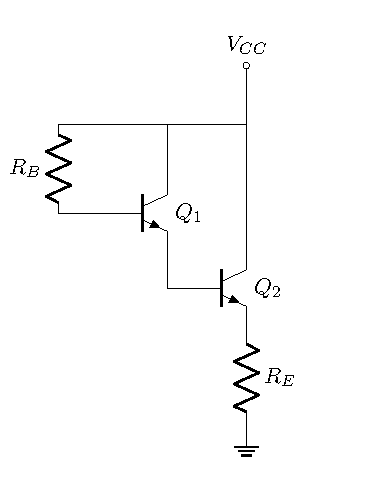
\includegraphics[width=0.5\textwidth, page=1]{Imagenes/ParDarlington.pdf}
	\caption{Par Darlington.}
	\label{fig:pardar1}
\end{subfigure}
\begin{subfigure}{.4\textwidth}
\centering
	\includegraphics[width=0.6\textwidth, page=2]{Imagenes/ParDarlington.pdf}
	\caption{Par Darlington compensado con $R$.}
	\label{fig:pardar2}
\end{subfigure}
\begin{subfigure}{.5\textwidth}
\centering
	\includegraphics[width=0.5\textwidth, page=3]{Imagenes/ParDarlington.pdf}
	\caption{Par Darlington compensado con fuente de corriente.}
	\label{fig:pardar3}
\end{subfigure}
\caption{Configuraciones posibles para el par Darlington.}
\label{fig:pardar}
\end{figure}

La conexión representada en la Figura (\ref{fig:pardar1}) no es conveniente ya que ambos transistores consumen mucha corriente. Estrictamente hablando, la disposición presentada en la Figura (\ref{fig:pardar2}) es la más económica. Dadas las condiciones, dicha consideración no afecta en la decisión a implementar, ya que se cuenta con componentes para realizar cualquiera de las tres. Finalmente, la mostrada en la Figura (\ref{fig:pardar3}) es más optima para compensar el circuito, ya que permite aumentar $I_{CEQ}$ sin modificar otros factores del propio circuito.
\begin{center}
	\LARGE{\textcolor{red}{Mejorar justificación de porqué a y b son peores que c.}}
\end{center}

\subsection{Fuente de corriente}
\label{subsec:fdei}
Una vez determinado que la implementación optima, con los componentes disponibles, es la presentada en la Figura~(\ref{fig:pardar3}), se decide confeccionarla. Para ello, primero se opta por analizar la fuente de corriente. Esta puede ser realizada con el JFET, dispuesto en una configuración en la cual se autopolarice, como se presenta a continuación.
\begin{figure}[H]
\centering
	\includegraphics[width=0.2\textwidth, page=4]{Imagenes/ParDarlington.pdf}
	\caption{Par Darlington.}
	\label{fig:fuentei}
\end{figure}

Recorriendo la malla de entrada y de salida del circuito de la Figura (\ref{fig:fuentei}), se obtienen las siguientes ecuaciones:
\begin{equation}
	V_{GS} = V_{SS} - I_{D} R_{S}
\end{equation}
\begin{equation}
	V_{DS} = V_{DD} + V_{SS} - I_{D} \left( R_{D} + R_{S} \right)
\end{equation}

Sabiendo que para un JFET se cumple que
\begin{equation}
\begin{split}
	I_D = I_{DSS} \left( 1- \frac{V_{GS}}{V_P} \right)^2 \\
	gm = 2\frac{\sqrt{I_D I_{DSS}}}{|V_P|}
\end{split}
\end{equation}

De esta forma, seleccionando el componente XX %\href{}{}
y estableciendo $V_{SS} = XX \ V$, $V_{DD} = XX \ V$, $R_S = XX \ \Omega$ y $R_D = XX \ \Omega$ se obtiene
\begin{center}
	\LARGE{\textcolor{red}{Poner que JFET se usó, datasheet y reemplazar valores.}} \\
	\LARGE{\textcolor{red}{Seleccionar que resistencias usar, $V_{SS}$ y $V_{DD}$.}}
\end{center}

Con lo establecido previamente, se prosigue a plantear el circuito incremental. Cabe aclarar que, como es de interés calcular la impedancia de salida, no se puede consideran tanto $R_{DS}$ como $R_{GS}$ despreciables. Es por ello que son tenidas en cuenta para este cálculo.
\begin{figure}[H]
\centering
	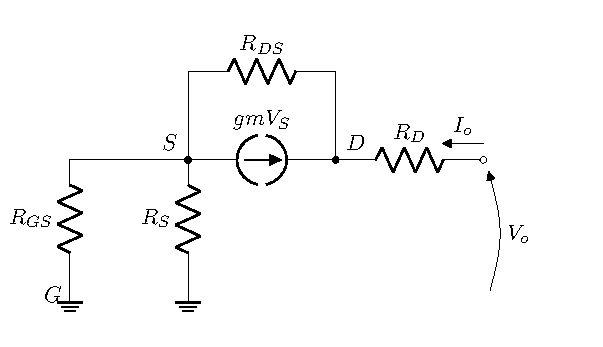
\includegraphics[width=0.5\textwidth, page=1]{Imagenes/ModeloIncremental.pdf}
	\caption{Circuito incremental de la Figura (\ref{fig:fuentei}).}
\label{fig:incfuente1}
\end{figure}

Se destaca que, como el Gate queda a tierra, se cumple que $V_{GS} = V_G - V_S = - V_S$, por lo tanto, se da vuelta la fuente de corriente y se reemplaza con lo mencionado anteriormente. 

Se define $R_S^* = R_S // R_{GS}$, para luego analizar el circuito presentado en la Figura (\ref{fig:incfuente2}).
\begin{figure}[H]
\centering
	\includegraphics[width=0.5\textwidth, page=2]{Imagenes/ModeloIncremental.pdf}
	\caption{Análisis de la impedancia de salida del circuito de la Figura (\ref{fig:incfuente1}).}
\label{fig:incfuente2}
\end{figure}

Planteando
\begin{equation*}
	I^* = \frac{V_S}{R_S^*}
\end{equation*}
\begin{equation*}
	V_o = -I^* R_D = -I_o R_D
\end{equation*}
\begin{equation*}
	I_{DS} = \frac{V_D - V_S}{R_{DS}}
\end{equation*}
y operando algebraicamente se obtiene la variable deseada de la forma:
\begin{equation}
	R_{OF} = R_{DS} \left( 1 + gm R_S^* \right) + R_S^*
\end{equation}

\subsection{Darlington polarizado por corriente}
Con lo obtenido en la Sección (\ref{subsec:fdei}), se posee la información necesaria para analizar el circuito presentado en la Figura (\ref{fig:pardar3}). El primer paso, consiste en reemplazar la fuente de corriente por su respectiva impedancia de salida $R_{OF}$.
\begin{figure}[H]
\centering
	\includegraphics[width=0.4\textwidth, page=5]{Imagenes/ParDarlington.pdf}
	\caption{Circuito equivalente al reemplazar la fuente de corriente.}
	\label{fig:pardar4}
\end{figure}

Planteando la malla de entrada y salida para cada transistor, se obtienen las siguientes ecuaciones:
\begin{equation*}
	V_{CC} - V_{BEON} = I_{CE1} R_{OF}
\end{equation*}
\begin{equation*}
	V_{CC} - 2V_{BEON} = I_{CE2} R_{OF}
\end{equation*}
\begin{equation*}
	V_{CC} - V_{CE1} = I_{CE1} R_{OF}
\end{equation*}
\begin{equation*}
	V_{CC} - V_{CE2} = I_{CE2} R_{C}
\end{equation*}

Cabe destacar que, por el uso de la fuente de corriente, $I_{CE1} = I_{D}$ del JFET. Además, se seleccionar transistores NPN XX
\begin{center}
	\LARGE{\textcolor{red}{Poner que NPNs se usaron, datasheet y reemplazar valores.}} \\
	\LARGE{\textcolor{red}{Seleccionar que resistencias usar, $V_{CC}$.}}
\end{center}

Planteando su respectivo modelo incrementa, se llega al circuito presentado a continuación: 
\begin{figure}[H]
\centering
	\includegraphics[width=0.8\textwidth, page=3]{Imagenes/ModeloIncremental.pdf}
	\caption{Modelo incremental del par Darlington.}
\label{fig:incdar}
\end{figure}

\subsection{Desarrollo y armado de la placa}

\subsection{Mediciones}

\section{Conclusiones}
	
\end{document}